\chapter{実験}
本章では提案手法であるSWMHと,バッチSWMHを人工データと実データを用いて実験的に評価する.6.1節で使用したデータセットを記述する.次に,6.2節ではデータストリームの到着レートが1である状況でSWMHを評価する.ここでは,時刻変化のたびにスライディングウインドウ全体をスキャンして,Min-hashのハッシュ値を再計算する手法をBaselineとし,SWMHがBaselineより高速であることを示す.6.3節ではデータストリームの到着レートが$c>1$である条件でバッチSWMHを評価する.ここでは,5.1節で述べたSWMHを$c$回適用する単純手法とバッチSWMHの実行時間を比較する.





\section{データセット}
\subsection{人工データセット}
人工データセットは,アルファベット$\phi$から,zipf分布に従ってサンプリングを繰り返し,長さ100,000の文字列$st$を生成する.
到着レートを$c$として,データストリームは$st$の先頭から順に毎時刻$c$個取り出すことで,シミュレートする.データセットの特性を決定するパラメータは
\begin{itemize}
\item $\alpha$ : zipf分布の偏りをコントロールするパラメータ
\item $\phi$ :アルファベットの種類数
\end{itemize}

であり,スライディングウインドウのの長さを $W$とする.
zipf分布とは,$\alpha$を$[0,1]$の範囲で指定し,アルファベットの出現頻度に偏りを持たせた分布である.アルファベットの出現順位を$k$,$k$番目のアルファベットの個数を$N_k$,一番出現頻度の高いアルファベットの個数を$N_{max}$とすると,zipf分布は以下の式\ref{eq:zipf}で表せる.

\begin{equation}
 \label{eq:zipf}
N_k = N_{max} \times 1/k^\alpha
\end{equation}

$\alpha$はzipf分布の偏りをコントロールするパラメータで$\alpha$が大きいほど出現頻度の偏りが大きい.その結果,$\alpha$が大きいほどスライディングウインドウ内の要素の多重度大きくなる.$\alpha = 0$の時は単に一様分布に従ってサンプリングがなされる.

\subsection{実データセット}
実データによる実験は,connect datasetとmushroom datasetの2種類のデータ \cite{Maxloghash} \cite{dataset2} からデータベースを作成した.まず,connect datasetとは117種類のラベルが出現し,約20の長さのラベルから成る集合が約4,000列連なったデータである.次に,mushroom datasetとは127種類のラベルが出現し,約20の長さのラベルから成る集合が約60,000列連なったデータである.どちらのデータも1つの集合に同じラベルは含まれないデータである.それらのデータからランダムに集合を1つ選ぶ処理を,選ばれた集合をつなげた長さがデータストリームの長さ$100,000 + $ウインドウサイズ $W$を超える長さになるまで行い,データストリーム$st$を生成する.人工データと同じように,到着レートを$c$として,データストリームは$st$の先頭から順に毎時刻$c$個取り出すことで,シミュレートする.

\section{SWMHの実験評価}
まず,人工データを使った評価主数を説明する.人工データのパラメータは以下の3つである.
\begin{itemize}
\item $\alpha$
\item $\phi$
\item $W$

\end{itemize}

$\alpha = 1$, $|\phi|=100$,$W = 100$という組み合わせをデフォルトパラメータとし,それぞれのパラメータを変更し,実験を行なった.

次に,実データを使った評価主数を説明する.実データのパラメータは,

\begin{itemize}
\item $W$
\end{itemize}

のみであり,$W = 100$をデフォルトパラメータとし,実験を行なった.

それぞれの実験において,実験のばらつきを減らすために,ハッシュ関数を10個生成し,SWMH10回の合計を実行時間とし,実験を行なった.


実験	1): ウインドウサイズ $W$を変えて実験

スライディングウインドウサイズ $W = 100, 500, 1000, 5000, 10000$と変えて,提案手法の実行速度と最小値候補リストMinlistの長さを計測した.
人工データ, connect, mushroomいずれのデータセットにおいても,SWMHがBaselineより圧倒的に早かった(図\ref{fig:jikken1_1},\ref{fig:jikken1_2} ,\ref{fig:jikken1_3}).SWMHの実行時間は,Baselineと比べて,W=100の時,約9倍,W=1000の時,約17倍,W=10000の時,約60倍となった.実行時間とWの関係をより詳しく調査するため人工データに対する実行時間を対数グラフで表現したものを図\ref{fig:jikken1_taisu}に表す.Baselineでは,実行時間がWに対してリニアに増加するのに対して,SWMHでは実行時間が$\log (W)$に比例して増加する.Baselineの実行時間が$W$に比例するのはMin-hashの計算時間がO$(W)$であるためである.一方,SWMHの実行時間はMinlistの長さに関係があると考えられる.そこでMinlistの長さを調べた結果を図\ref{fig:jikken1_ML}に表す.Minlistの長さは,毎時刻ごとのMinlistの長さの1時刻の平均を表している.

%スライディングウインドウサイズ $W = 100, 1000, 10000$と変えて,提案手法の実行速度と最小値候補リストMinlistの長さを計測した. 割り当て値は,5回ランダムに生成し,実行速度とMinlistの計測は5回の平均値である.

%結果は,図\ref{fig:jikken1_1},\ref{fig:jikken1_2} ,\ref{fig:jikken1_3}より,人工データ,connect dataset, mushroom datasetのいずれのデータでも,Baselineではウインドウが長くなるごとに,大幅に実行時間が伸びていき,$W=10000$の時は,$W=100$の時に比べて,約50倍ほどの時間がかかっていることがわかる.図\ref{fig:jikken1_ML}より, 提案手法では,$W=10000$の時,$W=100$の時に比べて,約5倍ほどの時間で実行できており,$W$が大きくなっても,Baselineより与えられた影響が少ないことがわかる.


\begin{figure*}[h]
    \begin{tabular}{cc}
      %---- 最初の図 ---------------------------
      \begin{minipage}[t]{0.5\hsize}
        \centering
        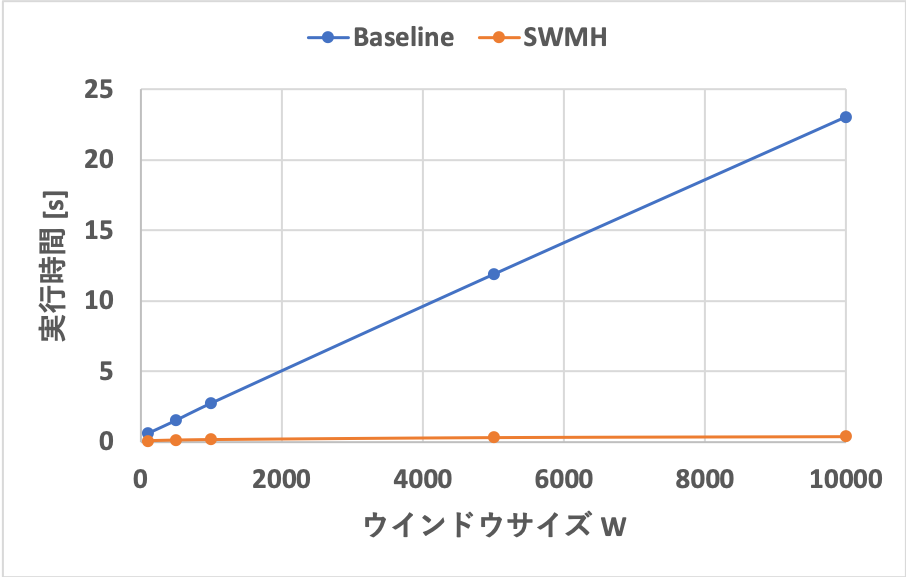
\includegraphics[width=8cm]{SW_jinko.png}
        \caption{人工 dataset}
        \label{fig:jikken1_1}
      \end{minipage}
      %---- 2番目の図 --------------------------
         \begin{minipage}[t]{0.5\hsize}
        \centering
        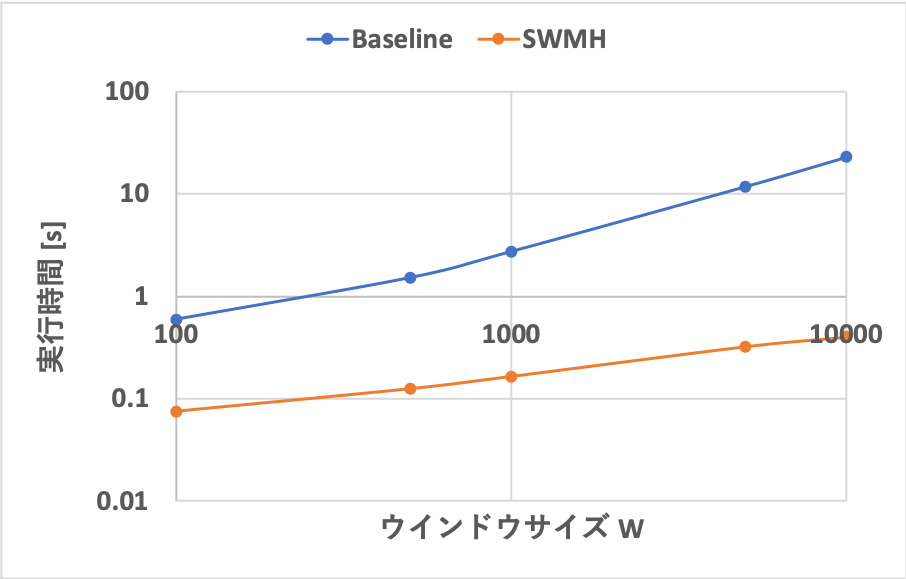
\includegraphics[width=8cm]{jikken1_1_taisu.png}
        \caption{人工datasetにおける対数グラフ}
          \label{fig:jikken1_taisu}
      \end{minipage}
      %---- 図はここまで ----------------------
    \end{tabular}
  \end{figure*}
  
   % \begin{figure*}[t]
  %\centering
  %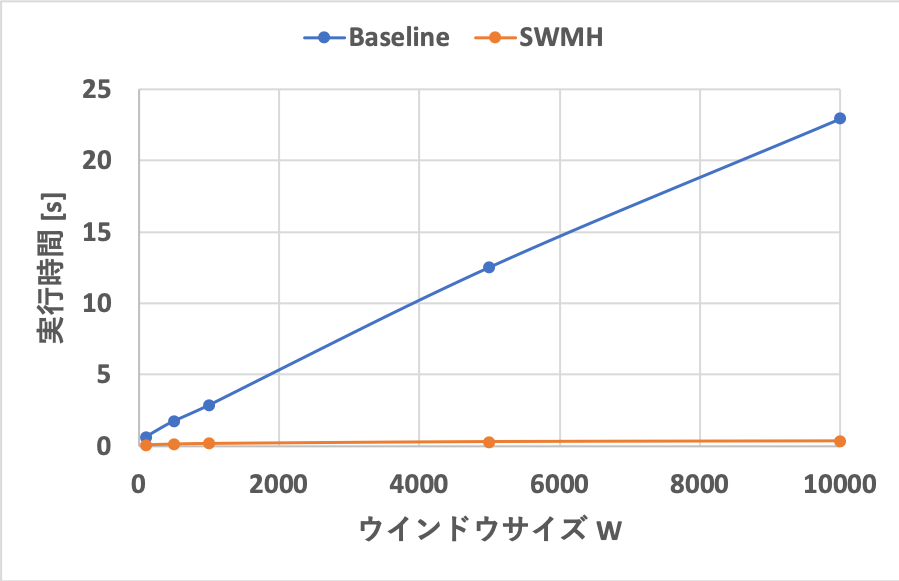
\includegraphics[width=8cm]{SW_connect.png}
    %\caption{connect dataset}
    %\label{fig:jikken1_3}
%\end{figure*}

\begin{figure*}[h]
    \begin{tabular}{cc}
      %---- 最初の図 ---------------------------
  \begin{minipage}[t]{0.5\hsize}
        \centering
        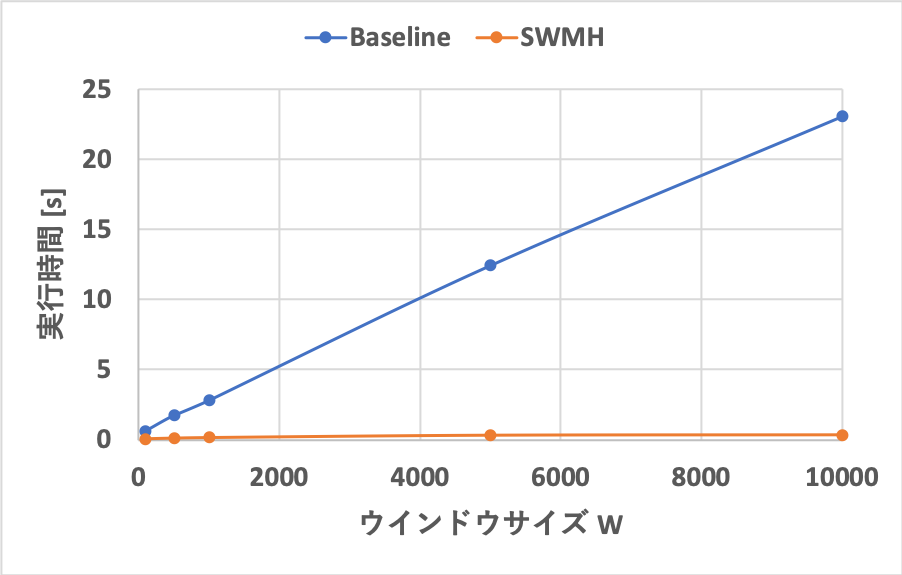
\includegraphics[width=8cm]{SW_mush.png}
        \caption{mushroom dataset}
          \label{fig:jikken1_2}
      \end{minipage}

      %---- 2番目の図 --------------------------
          \begin{minipage}[t]{0.5\hsize}
        \centering
        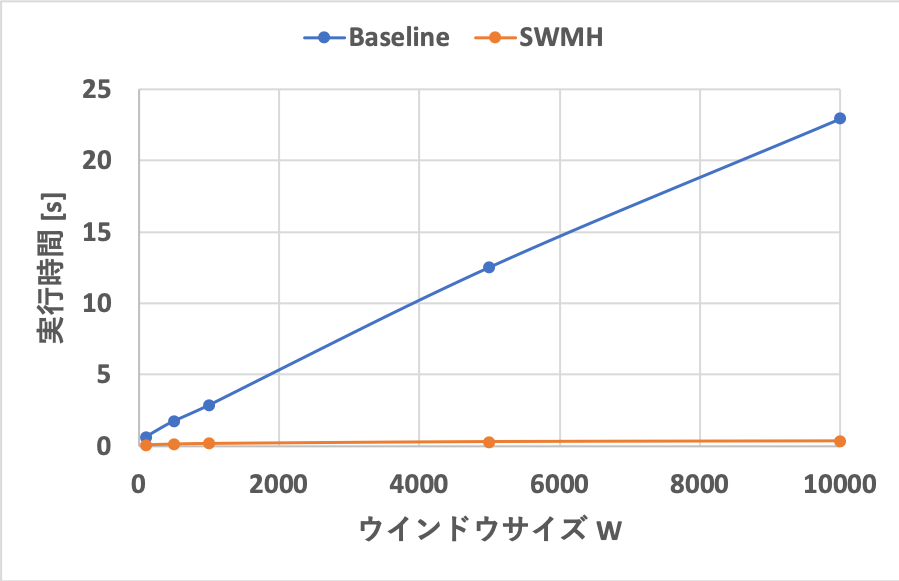
\includegraphics[width=8cm]{SW_connect.png}
      \caption{connect dataset}
    \label{fig:jikken1_3}
      \end{minipage}
         %---- 図はここまで ----------------------
    \end{tabular}
  \end{figure*}
  
  

      \begin{figure*}[h]
  \centering
  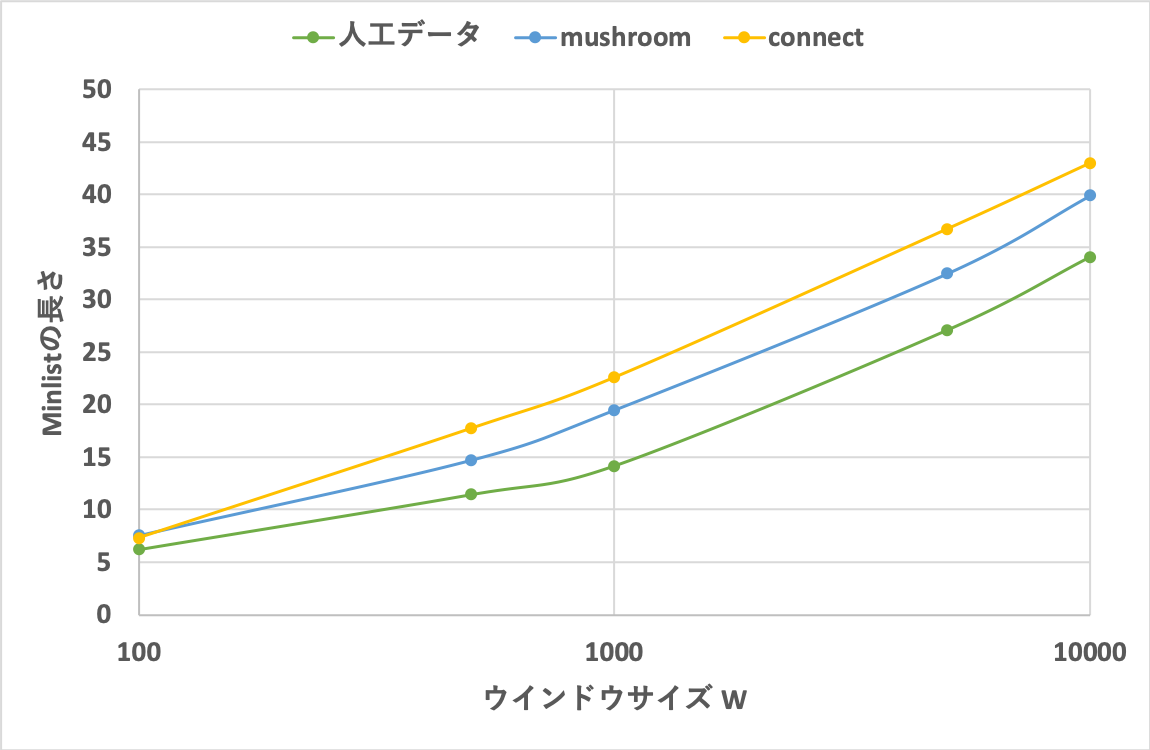
\includegraphics[width=14cm]{jikken1_SW.png}
    \caption{Wに対するMinlistの長さ}
    \label{fig:jikken1_ML}
\end{figure*}


実験 2):偏りパラメータ$\alpha$を変えて実験

偏り $\alpha = [0,1]$の幅で$0.1$ごとに変えて,SWMHの実行時間とMinlistの長さを計測した.%(図 \ref{fig:jikken2}).

人工データ, connect, mushroomいずれのデータセットにおいても,SWMHがBaselineより早かった(図\ref{fig:jikken2}).Baselineでは,偏りが大きくなるにつれて実行時間が短くなることに対して,SWMHでは実行時間が長くなっていく.これは,偏りが大きいほど要素の出現に偏りができ,ハッシュ値計算時の割り当て値表へのアクセスが局所的になり,キャッシュ効率が改善したためBaselineは実行時間が短くなったと考えられる.
しかし,SWMHでは,偏りが大きくなるごとに同じ要素が多く出やすくなる影響から4.2.3のアルゴリズムによりMinlistスキャンの際に,ヒストグラムや割り当て表を深く参照する回数が増える一方で,Minlistの長さに大きな影響を与えないため実行時間が長くなっていると考えられる.
%しかし,SWMHでは,偏りが大きいほどMinlist内で違うラベルを持つ要素より,同じラベルを持つ要素にMinlist内の要素は消され,更新されることが増える(図\ref{fig:same_another}).これは,同じラベルによりMinlistを更新する際に,ウインドウに含まれているラベルの要素数を保持しているヒストグラムにアクセスすることが増えるために,実行時間が遅くなっていくことが考えられる.
表\ref{tab:jikken2},図\ref{fig:same_another}より,Minlistの長さは,$\alpha$が増えるごと途中までは,増加するが,途中から減少する.これは,$\alpha$が大きくなるにつれて,Minlist内の要素が違うラベルによって消される減少量より,同じラベルに消される増加量が大きくなっていくことにより,起きていると考えられる.

%さらに,$\alpha = [0 ,1]$の幅で0.1ごとに変えて,提案手法の実行時間とMinlistの長さを計測した(表 \ref{tab:jikken2}).

%図 \ref{fig:jikken2} より,Baselineでは,偏りが上がるごとに実行時間が短くなることに対して,MHI4では実行時間が長くなっていく.これは,傾きが大きいほど,要素の出現に偏りができ,Baselineでは割り当て表へのアクセスが数箇所に集中し,時間が短くなったことが考えられる.しかし,提案手法では,傾きが大きいほどMinlist内で違うラベルを持つ要素より,同じラベルを持つ要素にMinlist内の要素は消され,更新されることが増える.これは,同じラベルによりMinlistを更新する際に,ウインドウに含まれているラベルの要素数を保持しているヒストグラムにアクセスすることが増えるために,実行時間が遅くなっていくことが考えられる.

 \begin{figure*}[h]
  \centering
  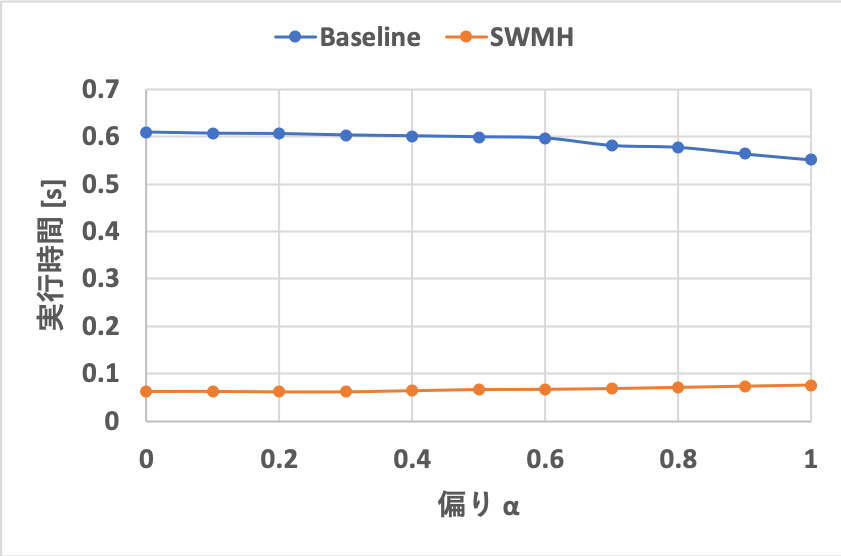
\includegraphics[width=14cm]{katamuki.png}
    \caption{傾き$\alpha$を変えた実行時間}
    \label{fig:jikken2}
\end{figure*}
  
  \begin{figure*}[h]
  \centering
  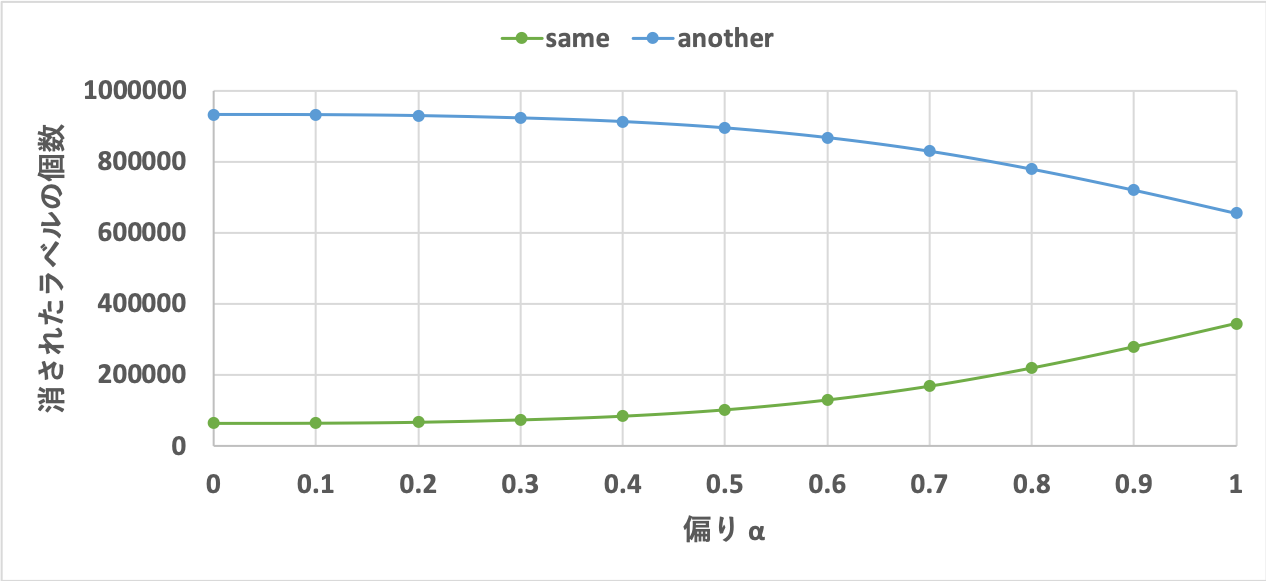
\includegraphics[width=14cm]{same_another.png}
    \caption{Minlistの消去されたラベルの種類}
    \label{fig:same_another}
\end{figure*}


\begin{table}[h]
 \caption{傾きと実行時間,Minlistの長さとの関係}
  \label{tab:jikken2}
 \centering
 \scalebox{0.8}{
  \begin{tabular}{|c| |r|r|r|r|r|r|r|r|r|r|r|}
 
   \hline
    傾き& 0 & 0.1 & 0.2  & 0.3 & 0.4 & 0.5 & 0.6 & 0.7 & 0.8 & 0.9 & 1\\
  
   \hline \hline
   実行時間[s] & 0.06311 & 0.0631 & 0.06227 & 0.06238 & 0.06454 & 0.0668 & 0.6732 & 0.06885 & 0.0711 & 0.07347 & 0.07577 \\
   \hline
   Minlistの長さ & 6.44605 & 6.46051 & 6.47262 & 6.52681 & 6.59502 & 6.66685 & 6.75032 & 6.81968 & 6.62904 & 6.54369 & 6.29902 \\
   \hline
 
  \end{tabular}
  }
\end{table}


実験 3):ラベル種類数$|\phi|$の変更

要素の種類数 $| \phi | = 10,50,100,500$と変えて,提案手法の実行速度と最小値候補リストMinlistの長さを計測した.
図\ref{fig:jikken3}より,Baselineでは,$|\phi|$が増加すると実行時間が増加する.この理由は,ラベルの種類数が多いほど,割り当て値表の広範囲にアクセスし,アクセスが局所的でなくなった結果,キャッシュ効率が限定的にないためと思われる.
一方で,SWMHでは,ラベルの種類数が増えるほど,Minlist更新の際に,同じラベルを持つ要素同士の削除が減少し,実行時間が減っていくと考えられる.


  \begin{figure*}[h]
  \centering
  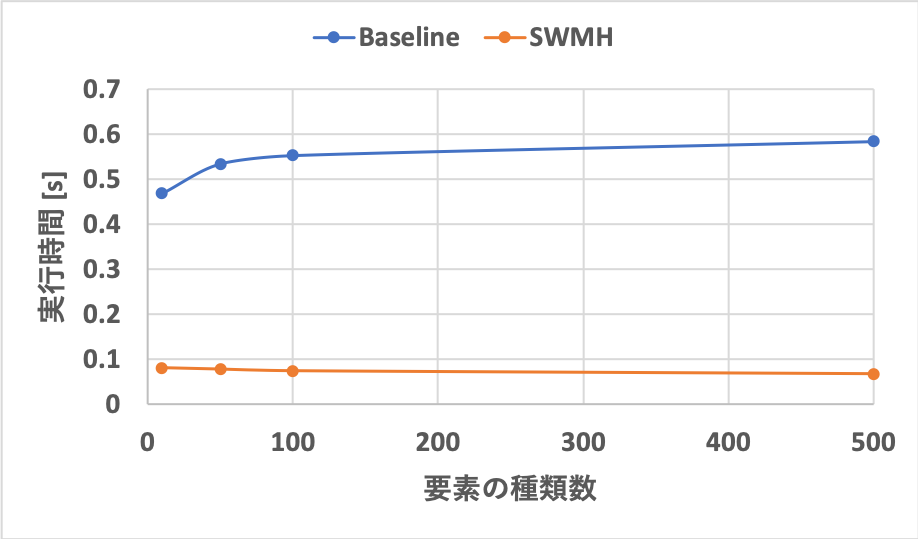
\includegraphics[width=14cm]{jikken3.png}
    \caption{ラベルの種類数$|\phi|$を変えた実行時間}
    \label{fig:jikken3}
\end{figure*}

実験4): ヒストグラム参照上限固定実験

SWMHのアルゴリズムでは,Minlistをスキャンする際に,スキャンされる要素$e'$よりウインドウ内で後ろにある$l(e_{t+1})$の個数に応じた$l(e_{t+1})$の割り当て値を使用し,将来必要ない要素の削除を行なっているが,ヒストグラムを参照する個数の上限を固定してMinlistをスキャンする実験を行う.例えば,上限2の場合,$e'$の後ろに$l(e_{t+1})$が5個あったとしても,$\pi(l(e_{t+1})_{5})$ではなく,$\pi(l(e_{t+1})_{2})$と比べて,$e'$を削除するか判定する.


参照するヒストグラムの個数を固定し,ラベルの種類数 $| \phi | = 10,30,100$と変えて,実行時間を計測した.
図\ref{fig:fix}より,$|\phi| = 10,30$の時は,ヒストグラム参照上限2で実行時間が一番短くなり,$|\phi| = 100$の時は,上限1の実行時間が一番短くなった.ヒストグラムを多く参照しても,Minlistの長さへ与える影響は少なくなり(図\ref{fig:fix_ML}),逆に何回も割り当て表やヒストグラムを参照することに時間をかけていると考えられる.

 \begin{figure*}[h]
  \centering
  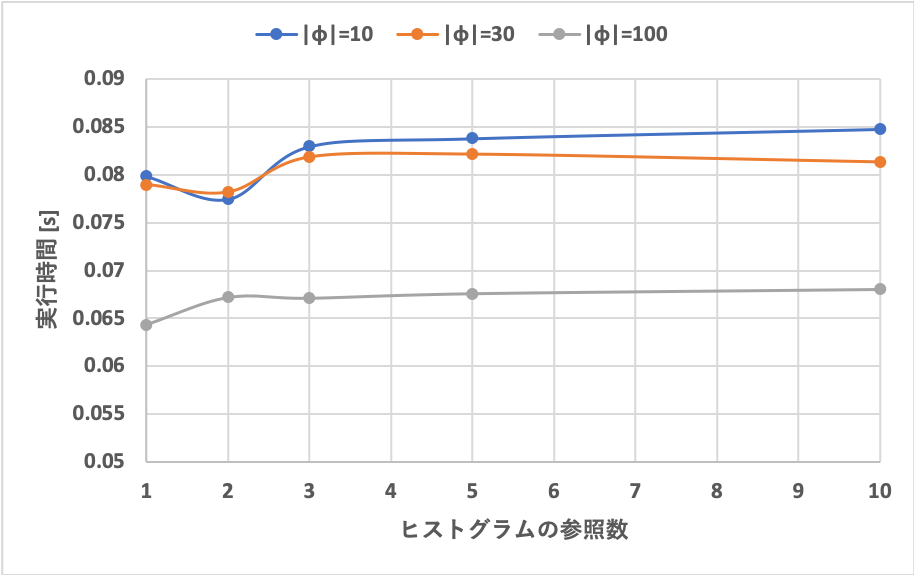
\includegraphics[width=14cm]{jikken_fix.png}
    \caption{ヒストグラムの参照数を変えた実行時間}
    \label{fig:fix}
\end{figure*}

 \begin{figure*}[h]
  \centering
  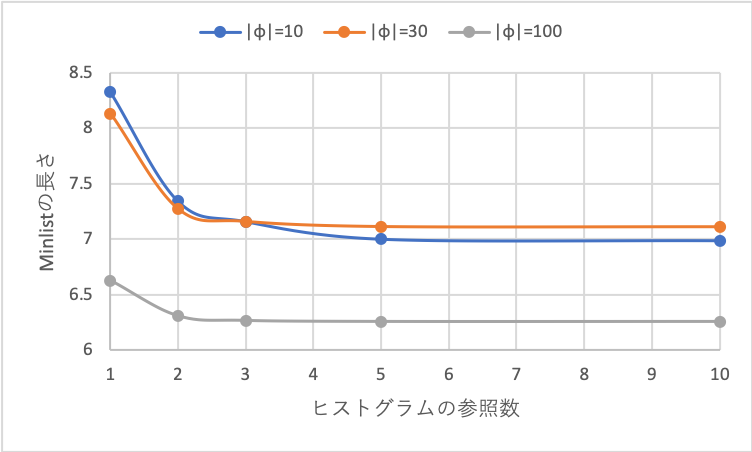
\includegraphics[width=14cm]{jikken_fix_ML.png}
    \caption{ヒストグラムの参照数を変えたMinlist}
    \label{fig:fix_ML}
\end{figure*}

\section{バッチSWMHの実験評価}
本実験では,人工データとconnect,mushroomの3つのデータセットを使用した.まず,人工データを使った評価主数を説明する.人工データのパラメータは到着レート$c = 5$,$\alpha = 1$, $|\phi|=100$,$W = 100$という組み合わせをデフォルトパラメータとし,実験を行なった.次に,実データを使った評価主数を説明する.実データのパラメータは,$c = 5$,$W=100$をデフォルトパラメータとし,実験を行なった.実験において,実験のばらつきを減らすためにハッシュ関数を10個生成し,バッチSWMHの合計を実行時間として,実験を行なった.

%実験 5): バッチSWMHの実行時間の計測
人工データ, connect, mushroomいずれのデータセットにおいても,SWMHを$c$回適応する方法より,バッチSWMHの方が約2倍早かった(表\ref{tab:jikken4_1} ).図\ref{tab:jikken4_2}より,Minlistの長さはバッチSWMHの方が長くなった.SWMHでは,c回スキャンするため,$c$個の要素のアルファベットを使用するが,バッチSWMHでは$c$個の要素のうち2個の要素のアルファベットのみを使用し,削除するためにMinlistが長くなっていると考えられる.しかし,入ってきた要素すべてとMinlist内の要素を比較して候補とならない要素を消していくのではなく,入ってきた要素の中から最小値となり得る要素を厳選し,その要素を用いて削除していくことによりMinlistを更新する回数を減らし,実行時間を短縮することができたと考えられる.


%SWMHとバッチSWMHを比較して実験し,バッチ SWMHの実行時間と最小値候補リストMinlistの長さを計測した.実験では,バッチSWMHのウインドウに一回に入ってくる要素数:5として実験を行なった(表\ref{tab:jikken4_1} ,表\ref{tab:jikken4_2}).
%実験結果より,SWMHより実行時間が短くなっていることがわかる.Minlistを更新する際に,入ってきた要素すべてとMinlist内の要素を比較して候補とならない要素を消していくのではなく,入ってきた要素の中から最小値となり得る要素を厳選し,その要素を用いて削除していくことによりMinlistを更新する回数を減らし,実行時間を短縮することができた.

\begin{table}[h]   
          \caption{バッチSWMHの実行時間}
        \label{tab:jikken4_1}
 \centering
  \begin{tabular}{|c| |c|c|c|}
   \hline
    データセット & 人工 & connect & mushroom\\
   \hline \hline
   SWMH & 0.0742 & 0.0743 & 0.073 \\
   \hline
   バッチSWMH & 0.042 & 0.0365 & 0.037 \\
   \hline
     \end{tabular}
  \end{table}
 
      
\begin{table}[h]
        \caption{バッチSWMHのMinlistの長さ}
          \label{tab:jikken4_2}
           \centering
  \begin{tabular}{|c| |c|c|c|}
   \hline
    データセット & 人工 & connect & mushroom\\
   \hline \hline
   SWMH & 6.2883 & 6.2082 & 6.296\\
   \hline
   バッチSWMH & 6.5501 & 7.5545 & 7.4214 \\
   \hline
    \end{tabular}
  \end{table}






